
\section{Results}
\label{sec:results}

In order to help the algorithm converge on the correct solutions, the parameters guiding the behavior of the algorithm were tailored to increase population diversity, maintain successful trees, and correctly adapt to the goal functions.  The sampling range of the functions also had significant impact on the algorithm's accuracy.  When comparing an expression tree to the goal functions, which determined the fitness of the trees, best results were seen when the error was calculated over a range where the goal function was significantly non-zero.  If the fitness was calculated over larger ranges of input values, the expression trees tended strongly towards constant expressions that minimize total error but describe only the asymptotic tails of the function.  

Data points taken from the first goal function are displayed in Table~\ref{tab:fcn1}.  The second goal function is four dimensional, and cannot be conveniently displayed.

\begin{figure}
\centering
	\begin{tikzpicture}
		\begin{axis}
			\addplot[scatter, only marks] table [x=x, y=y, col sep=space] {data1_small.txt};
		\end{axis}
	\end{tikzpicture}
\caption{Non-zero section of goal function 1}
\label{tab:fcn1}
\end{figure}

Despite careful adjustment of parameters governing tree construction, mutation rate, and the sampling range of the fitness function, we were unable to develop any non-constant expressions for the goal functions as given.  While closing the sampling range to only include the area of the fitness function displaying interesting, non-asymptotic behavior did result in lower error amongst the most accurate trees, the genetic algorithm was unable to determine a more accurate function.  

In order to attempt to match the first goal function, we inverted the output of the function in order to alter the expression needed to produce it.  Surprisingly, this met with success, as the algorithm consistently finds $x^2$ solutions which closely approximate the goal function.  Unlike the runs with the original goal function, the fitness scores converge when evaluating based on the inverted function.  Through this technique, we were able to arrive at an accurate function, which we then invert to conclude that the first goal function is 
	$$ y = \frac{10}{x^2- 6x + 14} $$

Unfortunately, this technique has not been successful for the second goal function, which has 3 input variables.  For that reason, we were also unable to plot the data in order to determine an appropriate sampling region or to visualize the function in general.  When attempting to fit the second goal function, our algorithm always relies on a constant function.  Unfortunately, this is clearly not a correct solution, as the error associated with such trees is massive.

%Present the results of your experiments. Simply presenting the data is
%insufficient! You need to analyze your results. What did you discover?
%What is interesting about your results? Were the results what you
%expected? Use appropriate visualizations. Prefer graphs and charts to
%tables as they are easier to read (though tables are often more
%compact, and can be a better choice if you're squeezed for space).
%\textbf{Always} include information that conveys the uncertainty in
%your measurements: mean statistics should be plotted with error bars,
%or reported in tables with a $\pm$ range. The $95\%$-confidence
%interval is a commonly reported statistic.

%\subsection{Embedding Pictures}
%\label{subsec:pics}

%See the source code (\texttt{results.tex}) for instructions on how to
%insert figures (like figure~\ref{fig:tex}) or plots into your
%document.

% Note that TeX has a mind of its own when it comes to placing images
% in documents - where a figure appears in the PDF document will often
% be quite different from where it appears in the source code. This is
% a feature, not a bug - it enables LaTeX to produce layouts that
% "flow" better. It only takes a few lines to insert a figure into
% your write-up - I recommend using PNG, JPG or PDF images
% (incidentally, programs like Excel and Matlab will allow you to save
% any plots or figures you generate in those formats). The \figure{}
% command is used to create a new figure.
%\begin{figure}[htb]

%  \centering  % centers the image in the column

  % replace the second argument below with your filename. I like to
  % place all my figures in a sub-directory to keep things organized
%  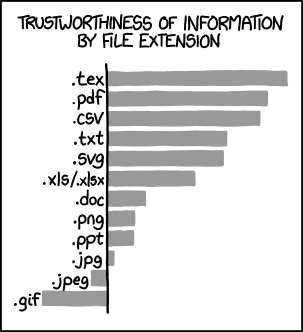
\includegraphics[width=0.47\textwidth]{figs/file_extensions.png}

  % *Every* figure should have a descriptive caption.
%  \caption{On the trustworthiness of \LaTeX. Image courtesy of \texttt{xkcd}.}

  % The label is a handle you create so that you can refer to this
  % figure (using the \ref{} command) from other parts of your
  % document. LaTeX automatically renumbers figures and updates
  % references when you recompile, so you should do it this way rather
  % than hard-coding in references. Notice that I've also been
  % creating labels for the various sections in the document; I could
  % use \ref{} command to refer to those sections using their labels
  % too.
%  \label{fig:tex}

%\end{figure}

%\subsection{Creating Tables}
%\label{subsec:tables}

%Again, refer to \texttt{results.tex} to learn how to create simple
%tables (like table~\ref{tab:example}).
%\begin{figure}[htb]
%  \centering % centers the entire table

  % The following line sets the parameters of the table: we'll have
  % three columns (one per 'c'), each
  % column will be centered (hence the 'c'; 'l' or 'r' will left or
  % right justify the column) and the columns
  % will have lines between them (that's the purpose of the |s between
  % the 'c's).
%  \begin{tabular}{|c|c|c|} 
%    \hline \hline % draws two horizontal lines at the top of the table
%    Column 1 & Column 2 & Column 3 \\ % separate column contents using the &
%    \hline % line after the column headers
%    $1$ & $3.1$ & $2.7$ \\
%    $42$ & $-1$ & $1729$\\
%    \hline \hline
%  \end{tabular}

  % As with figures, *every* table should have a descriptive caption
  % and a label for ease of reference.
%  \caption{An example table.}
%  \label{tab:example}

%\end{figure}

